\section{Experiment}
\label{experiment}
\subsection{Experimental Setup}

\begin{figure*}[!t]
\centering
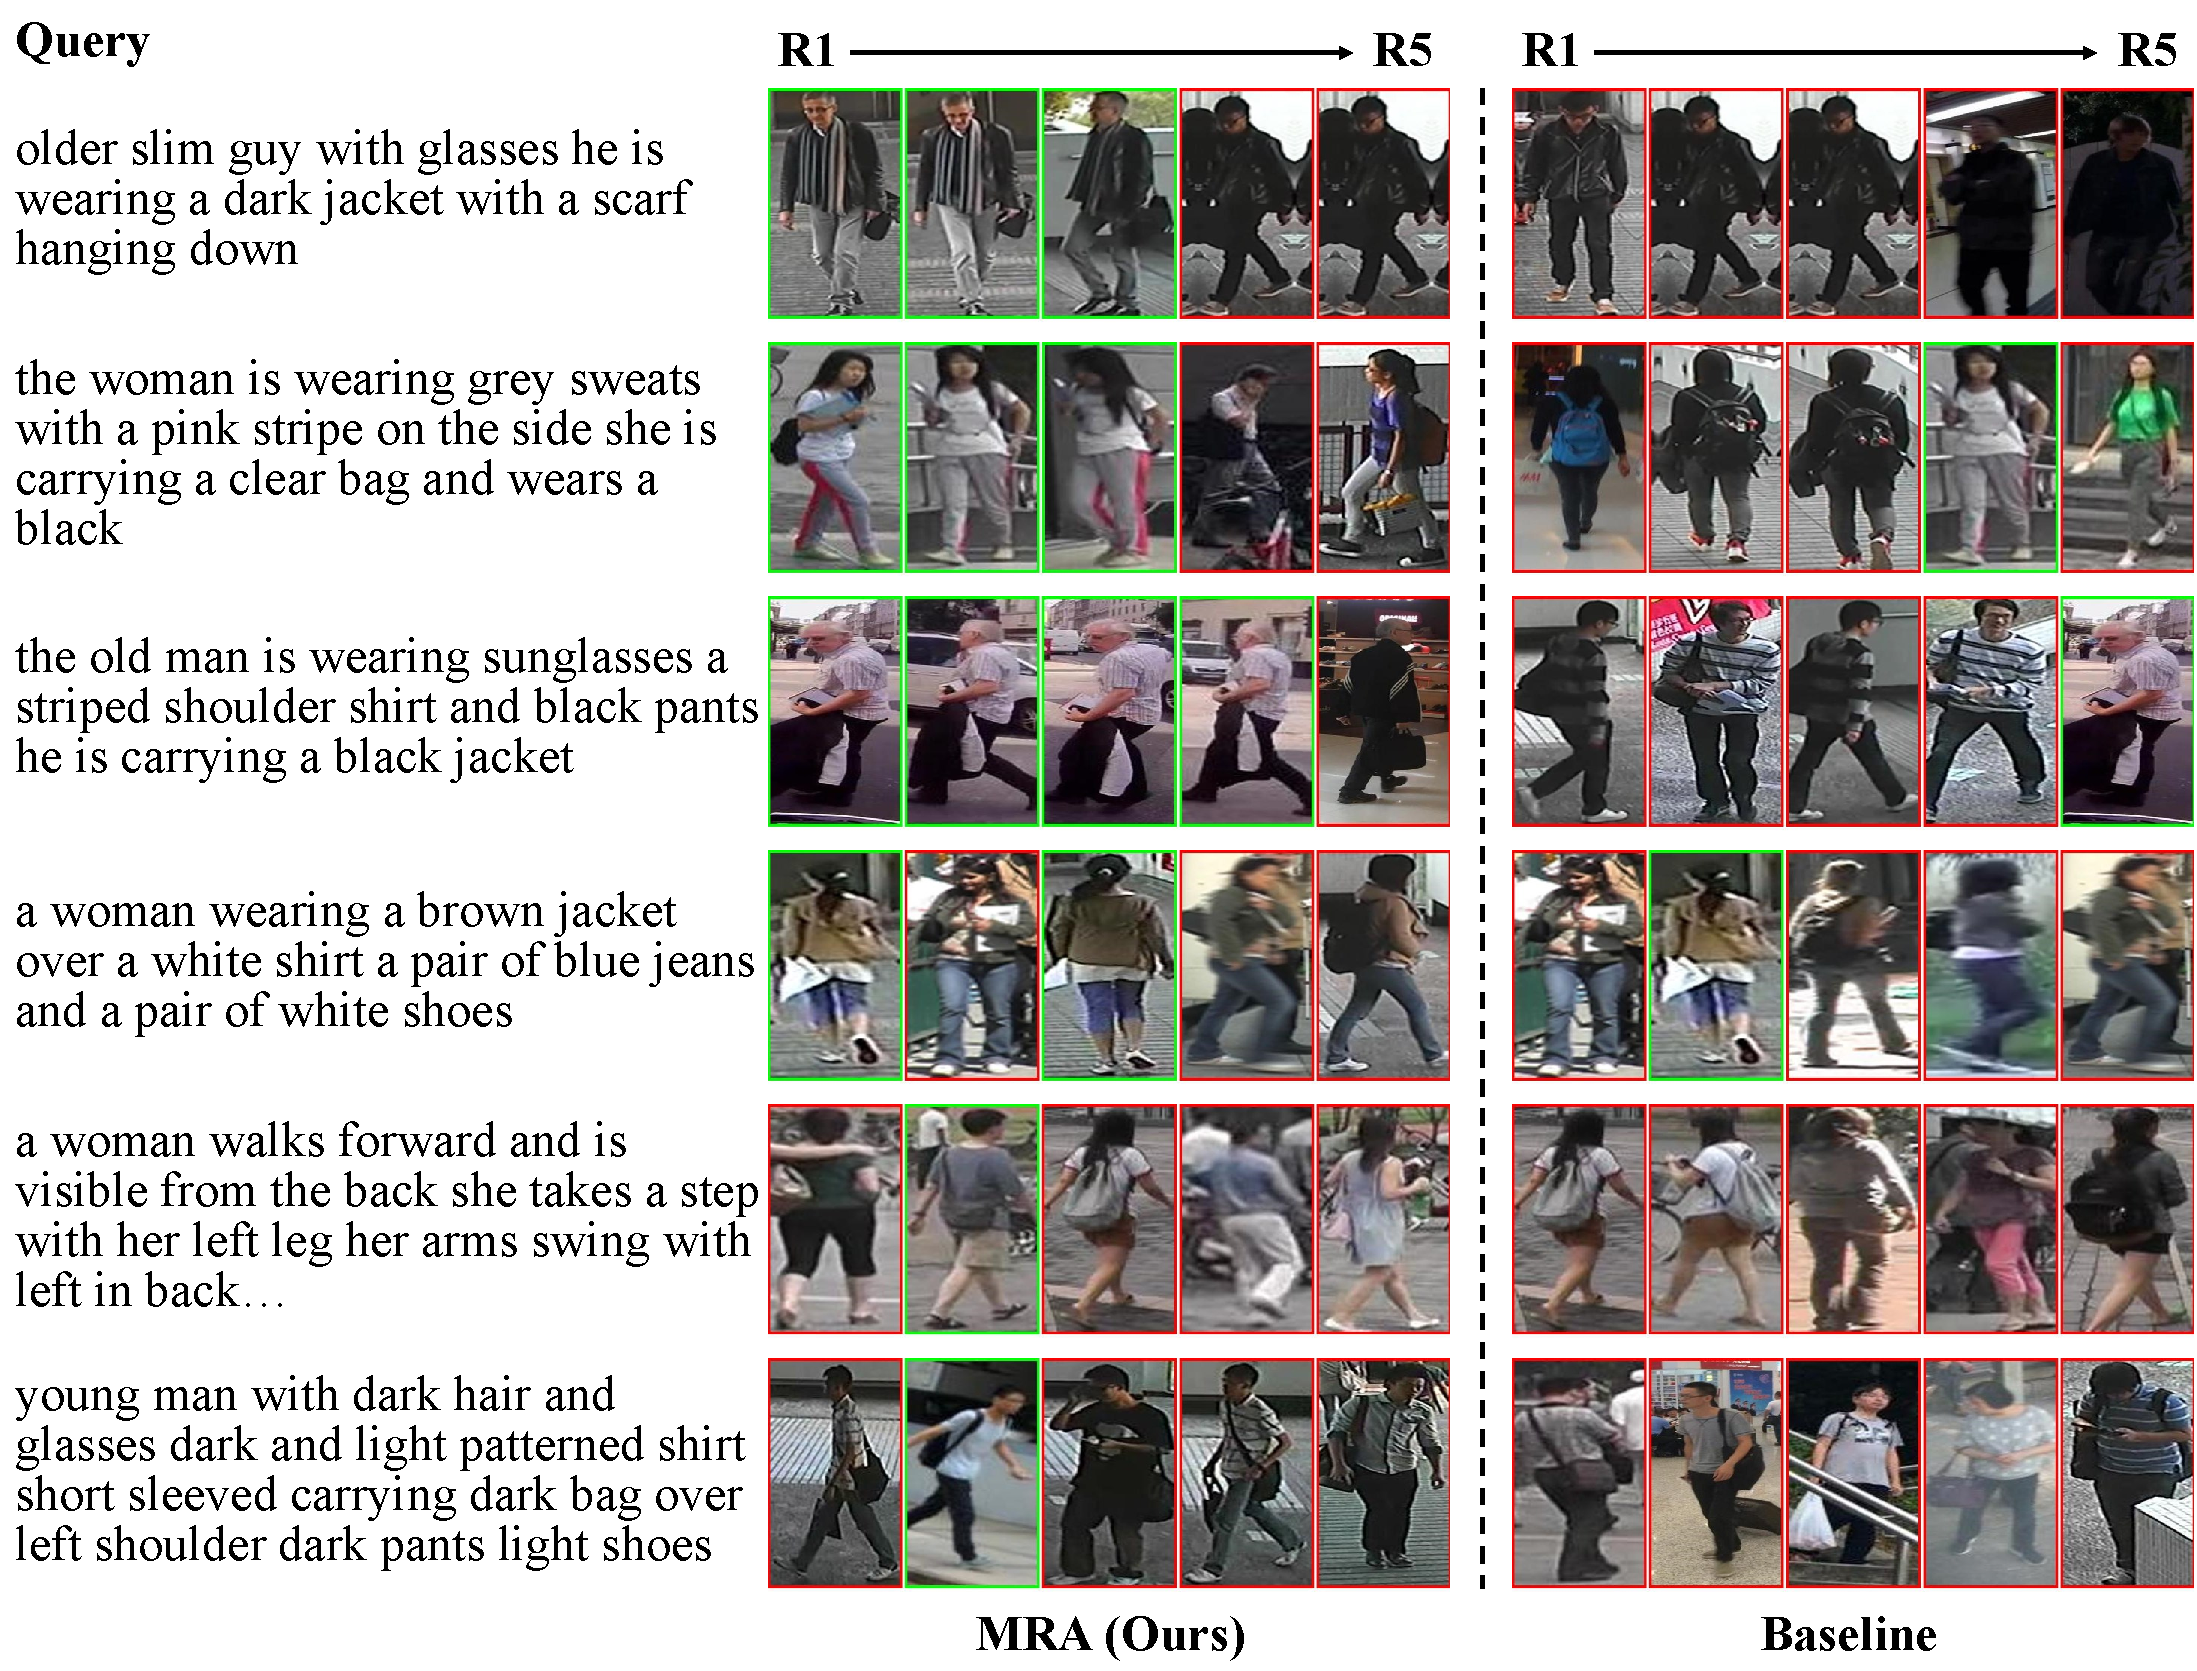
\includegraphics[width=0.72\linewidth]{images/results.pdf}
\caption{Qualitative text-based person retrieval results on CUHK-PEDES. The results are ranked from left to right in descending order of matching score. Green and red bounding boxes indicate correct and incorrect matches, respectively. 
The first four lines of retrieval results are success cases, while the bottom two lines are failures.
The proposed MRA method successfully recalls more true positives at the top rankings compared to the baseline. Notably, the failure cases of MRA are semantically reasonable, as the incorrect retrievals still correspond meaningfully to the text query.
}
\label{fig: result}
\end{figure*}

\noindent\textbf{Datasets.} 
\noindent We evaluate our approach on three public text-based person retrieval datasets, \ie, \textbf{CUHK-PEDES}~\cite{li2017person}, \textbf{ICFG-PEDES}~\cite{ding2021semantically}, and \textbf{RSTPReid}~\cite{zhu2021dssl}. 
In particular, \textbf{CUHK-PEDES}~\cite{li2017person} includes $80,440$ description sentences and $40,206$ photos of $13,003$ people. It is divided into three subsets: a training set that contains $34,054$ images and $68,126$ description sentences; a validation set that contains $3,078$ images and $6,158$ description sentences; and a testing set that contains $3,074$ images and $6,156$ description sentences. 
\textbf{ICFG-PEDES}~\cite{ding2021semantically} 
is incubated from MSMT17~\cite{wei2018person} and 
has $54,522$ images of $4,102$ individuals. There is an average of $37.2$ words in each description sentence for each image. The training subset has $34,674$ image-text pairs for $3,102$ people, whereas the testing subset has $19,848$ image-text pairs for the remaining $1,000$ people.
\textbf{RSTPReid}~\cite{zhu2021dssl} comprises $20,505$ images of $4,101$ people
and is also created by compiling MSMT17~\cite{wei2018person} data. 
Every image is associated with two sentences, each of which contains at least $23$ words. More specifically, there are $3,701$ IDs in the training set while $200$ and $200$ IDs in the validation and testing sets, respectively.  


\noindent\textbf{Evaluation Metrics.} 
For the text-based person retrieval, following earlier studies, we report recall rates, \eg, R@1, R@5,  R@10, and mAP.  The mean average precision (mAP) is the average area under the precision-recall curve across all queries. The higher Recall rate and mAP indicate better retrieval performance.


\noindent\textbf{Implementation Details.}
During pretraining, we optimize MRA with Pytorch on $4$ NVIDIA GeForce RTX 3090 GPUs for 32 epochs, and the mini-batch size is $40$. 
The learning rate is set to $5e^{-5}$ and is decayed to $5e^{-6}$ following a linear schedule, while the first $2600$ training iterations are performed as a warm-up. 
We use the AdamW~\cite{loshchilov2018decoupled} optimizer with a weight decay of $0.01$.
Before the training starts, the Vision Encoder, Text Encoder, and Fusion Encoder are initialized with Swin Transformer$_{\text{base}}$~\cite{liu2021swin}, the first six and the last six layers of BERT$_{base}$~\cite{devlin2019bert}, respectively. 
The trainable parameters of MRA are $226.5M$.
MRA adopts the image resolution of $224 \times 224$, while Random Horizontal Flipping and random Erasing are used to augment the image. 
The maximum text token length is set to $56$. 
Pretraining takes about 4 days.

\noindent\textbf{Fine-tuning Details.}
We fine-tune the model on the pedestrian retrieval datasets and only optimize ITC, ITM, and MLM.
During fine-tuning, we adopt $4$ NVIDIA A100 40GB GPUs to train the model for $30$ epochs with a mini-batch size of $40$. 
The learning rate following a linear schedule is equal to $1e^{-4}$ on CUHK-PEDES and ICFG-PEDES, $5e^{-5}$ on RSTPReid. 
The image is resized to $384 \times 256$ and we deploy Random Horizontal Flipping and Random Erasing for image data augmentation, while EDA~\cite{wei2019eda} for text data augmentation.




\begin{table*}[!t]
\caption{Performance Comparison on image-based person re-identification dataset Market-1501~\cite{zheng2015scalable}.
}
\label{tab: reid}
\small
\centering
\begin{tabular}{l|c|c|cccc}
\shline
Method & Pretraining Dataset & \# Data & R@1 & R@5 & R@10 & mAP \\
\hline
Swin Transformer   & ImageNet-1K~\cite{deng2009imagenet} & 1.28M & 91.12 & 96.62 & 98.22 & 76.31 \\
Swin Transformer & SDA & 1.22M & \textbf{94.39} & \textbf{97.86} & \textbf{98.63} & \textbf{84.26} \\
\shline
\end{tabular}
\end{table*}


\subsection{Comparison with Competitive Methods}
\noindent \textbf{Quantitative Results.} 
In this section, we present the results of the comparison with state-of-the-art methods on three person retrieval datasets. 
In other words, we adapt MRA for pedestrian retrieval and evaluate the effectiveness of our method on CUHK-PEDES, ICFG-PEDES, and RSTPReid datasets.
In reference, we first obtain the embeddings of all images and texts in the test set, followed by computing the image-to-text similarity. 
For each text, the top $512$ image candidates with the highest similarity to it are selected. 
Then the candidates are re-ranked by the Fusion Encoder. 
As shown in Table~\ref{tab:sota_CUHK}, \ref{tab:sota_ICFG}, \ref{tab:sota_RSTP}, our proposed method achieves SOTA recall rate on all three datasets. 
Note that the Baseline model denotes the model obtained without pretraining and training on the three datasets directly (only ITC, ITM, and MLM is optimized).
On CUHK-PEDES, the R@1, R@5, and R@10 of MRA are $77.21 \%$, $90.66 \%$, and $94.46 \%$ respectively, outperforming the second-place method APTM~\cite{yang2023towards} by $0.68 \%$, $0.64 \%$, and $0.31 \%$. 
Although our mAP is lower than RaSa~\cite{bai2023rasa}, this is because RaSa employs a mixed training strategy of strong and weak positive sample pairs. This strategy gives a larger boost to mAP. For a fair comparison with other methods, we do not use this strategy. As a reference, if we use the mixed training strategy for fine-tuning, the mAP can reach $72.14 \%$.
For ICFG-PEDES, we achieve $68.93 \%$ R@1, obtaining $0.42 \%$ and $3.65 \%$ improvements respectively compared to APTM~\cite{yang2023towards} and RaSa~\cite{bai2023rasa}, while all the other recall rates outperform previous methods.
On RSTPReid, we obtain $68.15 \%$ R@1, and $53.77 \%$ mAP, higher than all the other methods.
At the same time, our method has achieved competitive results, \ie, $86.30 \%$ R@5 and $91.10 \%$ R@10, compared to the previous two best methods. 






\begin{table}[!t]
\small
\centering
\caption{Comparison with other methods on the domain generalization task. We adopt CUHK-PEDES (denoted as C) and ICFG-PEDES (denoted as I) as the source domain and the target domain in turn.}
\renewcommand\arraystretch{1.2}
\setlength{\tabcolsep}{5pt}
\begin{tabular}{c|l|ccc}
\hline
                                                   & Method                            & R1        & R5       & R10          \\
\hline
\multirow{6}{*}{\rotatebox{90}{C $\rightarrow$ I}} & Dual Path \cite{zheng2020dual}    & 15.41     & 29.80      & 38.19       \\
                                                   & MIA \cite{niu2020improving}       & 19.35     & 36.78      & 46.42       \\
                                                   & SCAN \cite{lee2018stacked}        & 21.27     & 39.26      & 48.83       \\
                                                   & SSAN \cite{ding2021semantically}  & 29.24     & 49.00      & 58.53       \\
                                                   & LGUR \cite{shao2022learning}      & 34.25     & 52.58      & 60.85       \\
                                                   % & RaSa \cite{bai2023rasa}           & \textbf{50.59} & \textbf{67.46} & 74.09  \\
                                                   \cline{2-5}
                                                   & \textbf{MRA (Ours)} & \textbf{50.01} & \textbf{67.13} & \textbf{74.24}  \\
\hline\hline
\multirow{6}{*}{\rotatebox{90}{I $\rightarrow$ C}} & Dual Path \cite{zheng2020dual}    & 7.63      & 17.14      & 23.52       \\
                                                   & MIA \cite{niu2020improving}       & 10.93     & 23.77      & 32.39       \\
                                                   & SCAN \cite{lee2018stacked}        & 13.63     & 28.61      & 37.05       \\
                                                   & SSAN \cite{ding2021semantically}  & 21.07     & 38.94      & 48.54       \\
                                                   & LGUR \cite{shao2022learning}      & 25.44     & 44.48      & 54.39       \\
                                                   % & RaSa \cite{bai2023rasa}           & \textbf{50.70} & \textbf{72.40} & \textbf{79.58}  \\
                                                   \cline{2-5}
                                                   & \textbf{MRA (Ours)} & \textbf{47.66} & \textbf{68.70} & \textbf{76.82}  \\
                                                   
\hline
\end{tabular}
\label{tbl: dg}
\end{table}




\noindent \textbf{Qualitative Results.} 
We further provide qualitative text-based person retrieval results of our method and Baseline on CUHK-PEDES (see Fig.~\ref{fig: result}).
The four retrieval results at the top of the image represent successful cases, while the two retrieval results at the bottom are failure cases. Compared to the baseline, our method can distinguish finer-grained features and retrieve more matched person images. We observe that the mismatched images retrieved in failure cases generally still align broadly with the text query descriptions. This is primarily because real-world datasets are influenced by annotator subjectivity during the labeling process, making it challenging to comprehensively describe all characteristics of person images. 
To address this limitation, our future work will explore two directions: (1) leveraging large-scale Vision-Language Models (VLMs) for automated data augmentation to generate more diverse and fine-grained textual descriptions, and (2) designing noise-robust loss functions that can learn effectively from partially accurate or subjective annotations.



\begin{table}[!t]
\caption{Ablation Study on the SDA pretraining dataset on CUHK-PEDES. 
We report fine-tuned recall rates across different pretraining methods. * We reimplement the method with the official code.
}
\label{tab: sdaabl}
\footnotesize
\centering
\begin{tabular}{l|c|c|cc}
\shline
Method & Pretraining Dataset & \# Data & R@1 & R@10 \\
\hline
\multirow{4}{*}{IVT*~\cite{shu2022see}} 
& -                           & 0M    & 61.99 & 87.69 \\
& COCO~\cite{lin2014microsoft}, \etc. & 4M    & 63.56 & 88.86 \\
& MALS~\cite{yang2023towards} & 1.51M & 64.85 & 89.99 \\
& SDA                         & 1.22M & 65.35 & 89.90 \\
\hline
\multirow{2}{*}{APTM~\cite{yang2023towards}}
& -                           & 0M    & 66.44 & 90.76 \\
& MALS~\cite{yang2023towards} & 1.51M & 76.53 & 94.15 \\
\hline
\multirow{2}{*}{MRA (Ours)}
& -                           & 0M    & 71.23 & 92.43 \\
& SDA                         & 1.22M & \textbf{77.21} & \textbf{94.46} \\
\shline
\end{tabular}
\end{table}


\noindent \textbf{Domain Generalization.}
We conduct a series of domain generalization experiments to verify the generalization ability of MRA, following LGUR~\cite{shao2022learning}. As shown in Table \ref{tbl: dg}, we use models trained on the source domain to evaluate performance on the target domain. The CUHK-PEDES dataset and the ICFG-PEDES dataset serve as the source and target domains in turn. 
From CUHK-PEDES to ICFG-PEDES, MRA achieves SOTA results, \ie, $50.01 \%$ R@1, $67.13 \%$ R@5, and, $74.24 \%$ R@10, against other methods. 
On the task of domain generalization from ICFG-PEDES to CUHK-PEDES, MRA still outperforms all the other methods such as LGUR~\cite{shao2022learning} by a significant margin ($+22.22 \%$ R@1 improvement).



\begin{figure*}[!t]
\centering
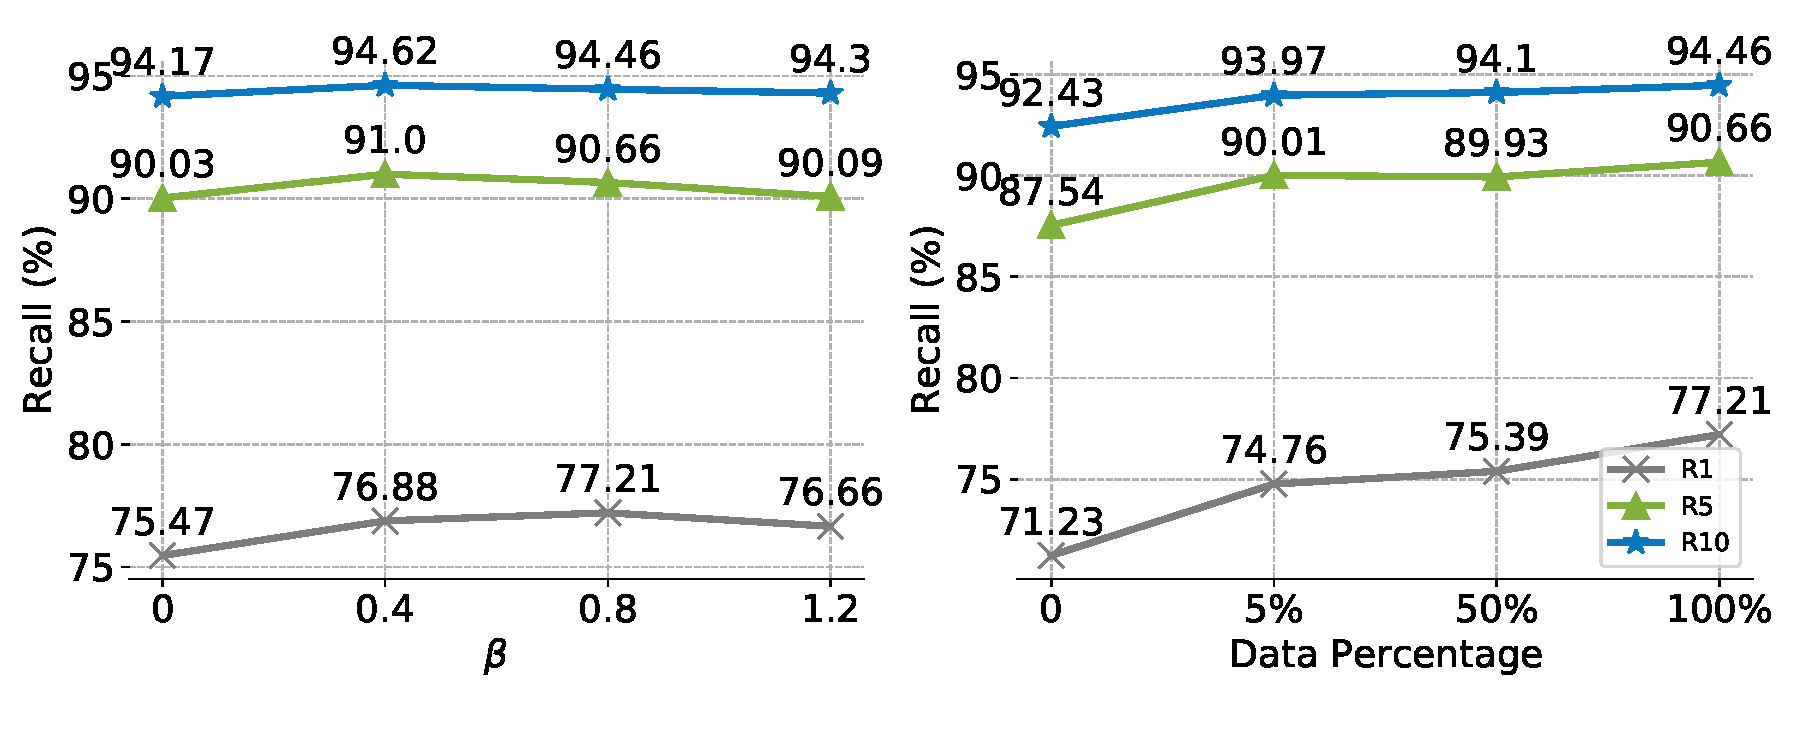
\includegraphics[width=0.72\linewidth]{images/beta_scale.pdf}
\caption{Ablation Study on $\beta$ and the pretraining data scale. In left subfigure, we set $\beta = \{0, 0.4, 0.8, 1.2\}$ respectively to validate the impact of $\beta$ on MRA. 
In right subfigure, we apply $0\%$, $5\%$, $50\%$, and $100\%$ data of SDA to pretrain. The fine-tuned recall rates on CUHK-PEDES are reported.  
}
\label{fig: beta_&_scale}
\end{figure*}


\noindent\textbf{Are SDA and MRA beneficial for image-based person re-identification?} 
We further evaluate the scalability of MRA on traditional image-based person re-identification tasks. 
Specifically, we compare the performance of the Swin Transformer (Swin-Base)~\cite{liu2021swin} pretrained on SDA (MRA Vision Encoder) with that pretrained on ImageNet-1K~\cite{deng2009imagenet} on the Market-1501~\cite{zheng2015scalable} dataset. 
As shown in Table~\ref{tab: reid}, under the same fine-tuning hyperparameter settings (image size: $224 \times 224$, fine-tuning epochs: 60), the MRA Vision Encoder achieves $94.39 \%$ R@1 and $82.46 \%$ mAP, outperforming the ImageNet-1K~\cite{deng2009imagenet} pretrained Swin Transformer by $+3.27\%$ R@1 and $+7.95 \%$ mAP. 
The experimental results show that the SDA dataset brings significant improvements to conventional image-based person re-identification, indicating strong robustness of MRA.






\begin{table}[!t]
\caption{Ablation Study on MRA loss on CUHK-PEDES. We apply $68,126$ data pairs from SDA to pretrain and then report the fine-tuned recall rate on CUHK-PEDES. $\mathcal{L}_{v1}$, $\mathcal{L}_{v2}$ and $\mathcal{L}_{v3}$ are losses of three variants of $\mathcal{L}_{MRA}$.
}
\label{tab: abl}
\footnotesize
\centering
\begin{tabular}{l|cccc|cc}
\shline
Method & $\mathcal{L}_{v1}$ & $\mathcal{L}_{v2}$ & $\mathcal{L}_{v3}$ & $\mathcal{L}_{MRA}$ & R@1 & R@10 \\
\hline
M1   & & & &              & 73.99 & 93.57 \\
M2   & $\checkmark$ & & & & 74.04 & 93.58 \\
M3   & & $\checkmark$ & & & 74.19 & 93.54 \\
M4   & & & $\checkmark$ & & 74.43 & 93.82 \\
\hline
MRA (Ours)  & & & & $\checkmark$ & \textbf{74.76} & \textbf{93.97} \\
\shline
\end{tabular}
\end{table}



\section{Ablation Studies}

\noindent \textbf{Effectiveness of Pretraining.} 
To validate the effectiveness of pretraining, we conduct a comprehensive empirical analysis on CUHK-PEDES. The experimental results are displayed in Table~\ref{tab: sdaabl}, where the accuracy of R@1 and R@10 is reported (To save space, R@5 and mAP are not reported).
The results in the last two rows of the table, \ie, the experimental results of Baseline \emph{VS.} MRA, show the impact of pretraining. After pretraining on SDA, MRA achieves $5.98 \%$ R@1 and $2.03 \%$ R@10 improvement. 
Similar results could be observed on ICFG-PEDES and RSTPReid, as shown in Table~\ref{tab:sota_ICFG} and Table~\ref{tab:sota_RSTP}. 
To intuitively show the advantages of pretraining, we present the qualitative comparison results of Baseline \emph{VS.} MRA in Figure~\ref{fig: result}.


\noindent \textbf{The Impact of SDA.} 
To further illustrate the superiority of SDA as a pretraining dataset, we compare it with MALS~\cite{yang2023towards}, a pedestrian image-text dataset with rich attribute annotations (used in APTM~\cite{yang2023towards}), and the general image-text datasets COCO~\cite{lin2014microsoft}, \etc, which contains four image caption datasets (refer to IVT~\cite{shu2022see} for details), totaling $4M$ image-text pairs. 
As shown in Table~\ref{tab: sdaabl}, pretraining on either MALS~\cite{yang2023towards} or SDA significantly improves retrieval accuracy. 
Notably, our MRA, pretrained on less data, outperforms APTM~\cite{yang2023towards} by $0.68\%$ in fine-tuned Recall@1.
Due to the architectural specificity of MRA and APTM~\cite{yang2023towards}, we further compare the pretraining datasets on IVT~\cite{shu2022see}, a general text-based person retrieval method that learns global image-text alignment without leveraging explicit attributes or local regions. 
For a fair comparison, we reproduce IVT~\cite{shu2022see} under our experimental setup. The results reported in Table~\ref{tab: sdaabl} are from our implementation.
The results show that IVT~\cite{shu2022see} pretrained on SDA achieves $65.35\%$ R@1, surpassing models pretrained on MALS~\cite{yang2023towards} and COCO~\cite{lin2014microsoft}, \etc.

\noindent\textbf{Effectiveness of MRA Loss.} 
MRA promotes the accuracy of pedestrian retrieval through multi-granularity relation alignment. 
For image-text level relation alignment, the effectiveness of ITC, ITM, and MLM among them has been demonstrated in previous work~\cite{jiang2023cross, bai2023rasa, yang2023towards} and will not be repeated in this paper. 
We focus on the effect of region-phrase level relation alignment.
In this part, the pretraining data scale is set to $68,126$ (the same as the training set of CUHK-PEDES). This setting is mainly for fair comparison and to avoid time-consuming experiments.
As shown in Table~\ref{tab: abl}, Method M1 only adopts image-text level relation alignment, without region-phrase level relation alignment.
The experimental results of our method and Method M1 indicate the performance improvement of MRA ($+0.77 \%$ R@1 and $+0.40 \%$ R@10). 
In other words, simultaneous relation alignment at multiple granularities during pretraining facilitates downstream pedestrian retrieval.
To further elucidate the effectiveness of our designed MRA, we compare it with three different variants. 
Specifically, we investigate the effects of image horizontal flipping in Grounding DINO, and finer-grained relation alignment, \ie, object-word level alignment. 
As shown in Table~\ref{tab: abl}, both variant 1 ($\mathcal{L}_{v1}$) and variant 3 ($\mathcal{L}_{v3}$) horizontally flip images at the rate of $50 \%$ in detecting objects and regions. 
For object-word level annotations, we use a string of the most frequently occurring words in CUHK-PEDES as the input prompt in Grounding DINO.
Variants 1 ($\mathcal{L}_{v1}$) and 2 ($\mathcal{L}_{v2}$) both conduct object-word level alignments, with the distinction that variant 2 utilizes only the bounding boxes without horizontally flipping in detecting objects. 
As shown in these experiments, leveraging region-phrase level (without horizontally flipping) annotations to conduct region-phrase level relation alignment yields better performance for cross-modal retrieval, with R@1 reaching $74.76\%$.

\noindent\textbf{Parameter Sensitivity of $\beta$.} 
To explore the effectiveness of the value of $\beta$ in Eq. \ref{eq: L_MRA}, we conduct further ablation experiments. 
We set $\beta$ to $0, 0.4, 0.8,  1, 2$ for pretraining separately and fine-tune the model on CUHK-PEDES. 
As shown in the left figure of Fig.~\ref{fig: beta_&_scale}, if $\beta = 0.4$ or $0.8$, the performance of the model is better. Intuitively, we set $\beta = 0.8$ without loss of generality.





\noindent\textbf{The Impact of Pretraining Scale.} 
The size of the pretraining dataset typically affects the performance of the pretrained model. Increasing the size of the data used in pretraining generally leads to varying degrees of improvement on downstream tasks, whether it is a general vision language pretraining model~\cite{radford2021learning, li2021align} or a text-based pedestrian retrieval pretraining model~\cite{yang2023towards}. In this paper, we further investigate the effect of the SDA scale on the pedestrian retrieval task. Specifically, we conduct ablation experiments varying the size of SDA, with pretraining data amounts set to $0 \%$ (no pretraining), $5 \%$, $50 \%$, and $100 \%$ of SDA, respectively. As shown in the right figure of Fig.~\ref{fig: beta_&_scale}, increasing the amount of pretrained data leads to improvements in the recall rate in line with previous research. Notably, there is a significant improvement in fine-tuning performance from $0 \%$ to $5 \%$, while the rate of performance improvement decreases from $5 \%$ to $100 \%$.
Our experiments indicate that a model pretrained on merely $5\%$ of the data achieves approximately $97\%$ of the performance achieved after fine-tuning on the downstream task. We attribute this phenomenon to the high degree of diversity and representativeness inherent in a small, randomly sampled subset of our pretraining corpus. Analysis reveals that this subset comprehensively covers the vast majority of person attributes, background, and linguistic structures present in the full SDA dataset. Furthermore, the pretraining dataset was deliberately constructed through domain adaptation to align closely with the target downstream CUHK-PEDES dataset, resulting in a high degree of domain correlation. Consequently, the feature representations learned from this limited pretraining data are already highly transferable and sufficient for effective adaptation to the target tasks.





